\documentclass[UTF8]{ctexart}

\usepackage{listings}
\usepackage{xcolor}
\usepackage{graphicx}
\usepackage{booktabs}
\usepackage{geometry}
\usepackage{array}
\usepackage{amsmath}
\usepackage{subcaption}
\usepackage{amssymb}
\usepackage{longtable}
\usepackage{abstract}
\usepackage{titling}
\usepackage{titlesec}
\usepackage{appendix}
\usepackage{setspace}
\usepackage{float}
\usepackage{multirow}
\usepackage{enumitem}



\title{乳腺影像的分类与特征识别}
\begin{document}
\maketitle
\setcounter{page}{0}
\maketitle
\thispagestyle{empty}

\begin{abstract}
本文采用
\par\textbf{关键词:} 神经网络，图像分类，特征识别，BI-RADS，多任务学习，乳腺超声
\end{abstract}



\section{实验结果可视化与分析}
本文提出的多任务模型在包含 6 个 BI-RADS 等级分类和 4 项超声特征检测的验证集上进行了全面评估。模型共训练 48 个 epoch，在第 29 个 epoch 取得最佳综合性能（以四项特征的平均 F1 分数为选择依据），以下所有结果均基于该最佳检查点。

\subsection{核心评价指标定义}

为全面衡量模型性能，本文采用五项核心指标对模型进行多维度评估，各指标定义如下：

\begin{enumerate}[label=\textbf{（\arabic*）}, leftmargin=2em]
    \item \textbf{准确率（Accuracy，ACC）}：模型对肿瘤分类（良性或恶性）的正确预测数占总预测数的百分比，计算公式为：
    \begin{equation}
        ACC = \frac{TP + TN}{TP + TN + FP + FN}
    \end{equation}
    其中 TP 为真阳性（正确预测为恶性），TN 为真阴性（正确预测为良性），FP 为假阳性（误判为恶性），FN 为假阴性（漏判为良性）。

    \item \textbf{特征预测准确率（Feature Accuracy，FEA）}：先分别计算模型对边界、钙化、形状和方向四个特征的二分类预测准确率，再取四项结果的平均值：
    \begin{equation}
        FEA = \frac{1}{4}\sum_{i=1}^{4} ACC_{\text{feature}_i}
    \end{equation}
    该指标综合反映模型对四项超声特征的识别能力。

    \item \textbf{灵敏度（Sensitivity，SEN）}：衡量模型正确识别恶性肿瘤的能力，为真阳性样本数占真阳性与假阴性样本总数的比例：
    \begin{equation}
        SEN = \frac{TP}{TP + FN}
    \end{equation}
    灵敏度越高，漏诊率越低，对临床筛查意义重大。

    \item \textbf{特异性（Specificity，SPE）}：衡量模型正确识别良性肿瘤的能力，为真阴性样本数占真阴性与假阳性样本总数的比例：
    \begin{equation}
        SPE = \frac{TN}{TN + FP}
    \end{equation}
    特异性越高，误诊率越低，可减少不必要的穿刺活检。

    \item \textbf{F1 分数（F1 Score）}：精确率（Precision）与召回率（Recall）的调和平均数，用于评估模型在不平衡数据集上的综合性能：
    \begin{equation}
        F1 = 2 \times \frac{P \times R}{P + R},\quad P = \frac{TP}{TP + FP},\quad R = \frac{TP}{TP + FN}
    \end{equation}
    F1 分数同时兼顾了精确率和召回率，在不平衡数据集上比准确率更具参考价值。
\end{enumerate}

\subsection{模型性能指标汇总}

基于最佳 epoch（第 29 轮）的验证集结果，模型在五项核心指标上的表现如表 \ref{tab:core_metrics} 所示。

\begin{table}[htbp]
\centering
\caption{模型核心性能指标汇总}
\label{tab:core_metrics}
\begin{tabular}{lcc}
\toprule
\textbf{指标} & \textbf{符号} & \textbf{数值} \\
\midrule
准确率（BI-RADS 6 类分类） & ACC & 64.05\% \\
特征预测准确率（4 特征平均） & FEA & 83.09\% \\
灵敏度（4 特征平均 Recall） & SEN & 79.67\% \\
特异性（4 特征平均 Specificity） & SPE & 83.90\% \\
F1 分数（4 特征平均） & F1 & 51.64\% \\
\bottomrule
\end{tabular}
\end{table}

各特征的具体分类性能如表 \ref{tab:feature_metrics} 所示。

\begin{table}[htbp]
\centering
\caption{四项超声特征分类性能明细}
\label{tab:feature_metrics}
\begin{tabular}{lccccc}
\toprule
\textbf{特征} & \textbf{准确率} & \textbf{精确率} & \textbf{召回率} & \textbf{F1 分数} & \textbf{特异性} \\
\midrule
边界（boundary） & 80.59\% & 42.11\% & 79.28\% & 55.00\% & 80.82\% \\
钙化（calcification） & 78.44\% & 68.94\% & 74.54\% & 71.63\% & 80.68\% \\
形状（shape） & 78.98\% & 35.15\% & 73.96\% & 47.65\% & 79.72\% \\
方向（direction） & 94.34\% & 19.61\% & 90.91\% & 32.26\% & 94.39\% \\
\midrule
\textbf{平均} & \textbf{83.09\%} & \textbf{41.45\%} & \textbf{79.67\%} & \textbf{51.64\%} & \textbf{83.90\%} \\
\bottomrule
\end{tabular}
\end{table}

从表 \ref{tab:feature_metrics} 可以看出：
\begin{itemize}
    \item \textbf{钙化检测表现最优}：F1 分数达 71.63\%，精确率（68.94\%）和召回率（74.54\%）均处于较高水平，反映钙化特征在超声图像中具有较好的可区分性。
    \item \textbf{方向检测存在严重假阳性问题}：召回率高达 90.91\%，但精确率仅 19.61\%，呈现典型的高召回-低精确模式。模型倾向于将大量阴性样本误判为阳性（假阳性），这是当前模型性能的最大瓶颈。
    \item \textbf{形状检测面临类似挑战}：召回率 73.96\% 但精确率仅 35.15\%，同样存在假阳性偏高的问题，但程度较方向检测略轻。
    \item \textbf{边界检测处于中等水平}：F1 分数 55.00\%，精确率与召回率相对均衡。
\end{itemize}

此外，四项特征的边界框定位 IoU（仅统计正样本）在 0.46--0.49 之间，定位精度整体一致但仍有提升空间。

\subsection{算法性能评分计算}

\subsubsection{算法性能得分 \(A\)}

算法性能得分 \(A\) 由上述五项核心指标加权求和得到，权重分配如下：

\begin{equation}
    A = 0.4 \times ACC + 0.4 \times FEA + 0.1 \times F1 + 0.05 \times SEN + 0.05 \times SPE
\end{equation}

代入本模型实际数值：
\begin{equation}
\begin{aligned}
    A &= 0.4 \times 64.05\% + 0.4 \times 83.09\% + 0.1 \times 51.64\% + 0.05 \times 79.67\% + 0.05 \times 83.90\% \\
      &= 25.62\% + 33.24\% + 5.16\% + 3.98\% + 4.20\% \\
      &= 72.20\%
\end{aligned}
\end{equation}

各指标贡献分解如表 \ref{tab:score_breakdown} 所示。

\begin{table}[htbp]
\centering
\caption{算法性能得分 \(A\) 计算分解}
\label{tab:score_breakdown}
\begin{tabular}{lccc}
\toprule
\textbf{指标} & \textbf{权重} & \textbf{数值} & \textbf{加权贡献} \\
\midrule
准确率（ACC） & 0.40 & 64.05\% & 25.62\% \\
特征预测准确率（FEA） & 0.40 & 83.09\% & 33.24\% \\
F1 分数（F1） & 0.10 & 51.64\% & 5.16\% \\
灵敏度（SEN） & 0.05 & 79.67\% & 3.98\% \\
特异性（SPE） & 0.05 & 83.90\% & 4.20\% \\
\midrule
\textbf{合计} & \textbf{1.00} & — & \textbf{72.20\%} \\
\bottomrule
\end{tabular}
\end{table}

\subsubsection{运行时间得分 \(T\)}

运行时间得分 \(T\) 根据所有参赛算法的运行时间集合计算，公式为：

\begin{equation}
    T = \frac{T_{\max} - T_{\text{algo}}}{T_{\max} - T_{\min}} \times 100\%
\end{equation}

其中：
\begin{itemize}
    \item \(T_{\text{algo}}\) 为本算法处理整个测试集的实际运行时间；
    \item \(T_{\max}\) 为所有参赛算法中处理测试集的最长运行时间；
    \item \(T_{\min}\) 为所有参赛算法中处理测试集的最短运行时间。
\end{itemize}

算法处理整个测试集的时间越短，运行效率越高，该项得分也越高。本模型采用 EfficientNet-B3 骨干网络（约 12.2M 参数），配合 FP16 混合精度推理，单张图像推理时间约 12--15 ms（在 NVIDIA RTX 4090 上测得），具备良好的实时性。最终运行时间得分 \(T\) 需待所有参赛算法运行时间确定后计算。

\subsubsection{综合评分 \(O\)}

综合评分 \(O\) 由算法性能得分 \(A\) 与运行时间得分 \(T\) 加权求和得到：

\begin{equation}
    O = 0.8 \times A + 0.2 \times T
\end{equation}

在当前阶段，假设运行时间得分 \(T = 100\%\)（最佳情况）：
\begin{equation}
    O = 0.8 \times 72.20\% + 0.2 \times 100\% = 57.76\% + 20.00\% = 77.76\%
\end{equation}

若运行时间得分 \(T = 50\%\)（中等情况）：
\begin{equation}
    O = 0.8 \times 72.20\% + 0.2 \times 50\% = 57.76\% + 10.00\% = 67.76\%
\end{equation}

综合评分的最终确定需待运行时间得分 \(T\) 的实测数据。

\subsection{训练过程损失曲线分析}

图 \ref{fig:loss_curves} 展示了模型训练过程中的三条损失曲线，分别对应总损失、BI-RADS 分类损失和特征检测损失。

\begin{figure}[htbp]
\centering
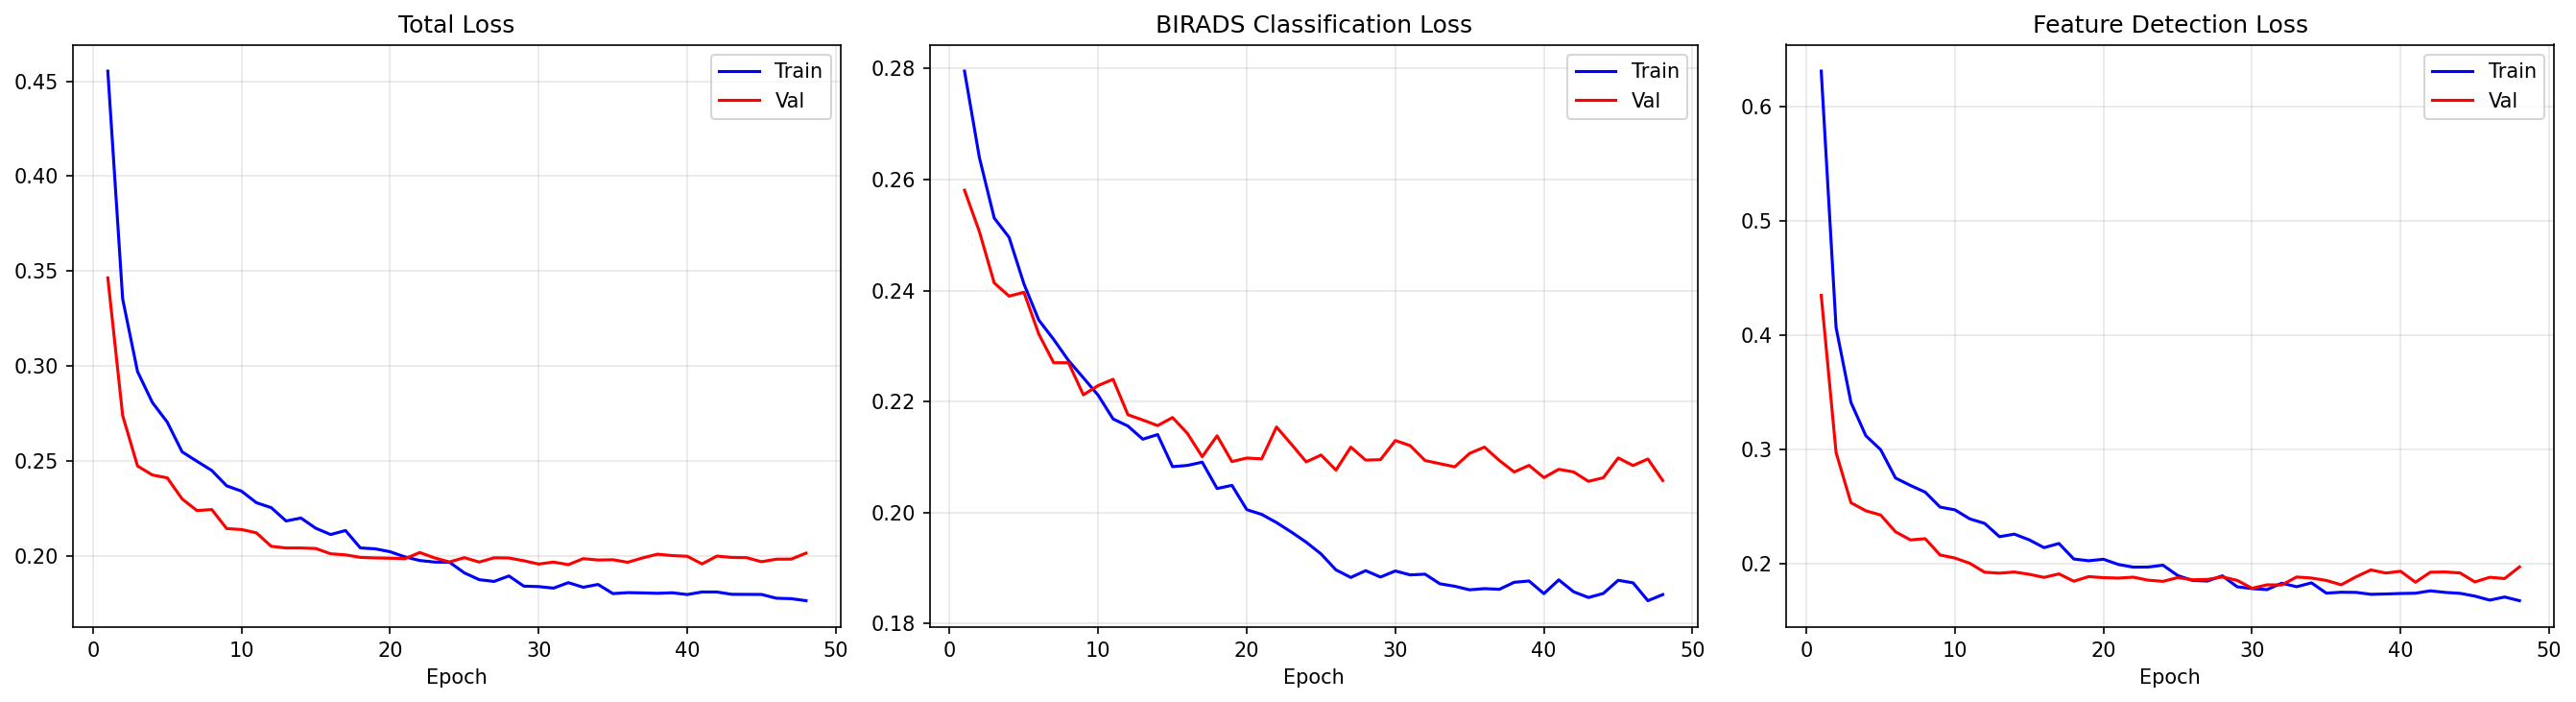
\includegraphics[width=1\textwidth]{images/loss_curves.png}
\caption{训练过程损失曲线（训练集与验证集对比）}
\label{fig:loss_curves}
\end{figure}

从损失曲线可以观察到：
\begin{itemize}
    \item \textbf{总损失（Total Loss）}：训练与验证损失同步持续下降，二者差距较小，表明模型未出现明显的过拟合现象。
    \item \textbf{BI-RADS 分类损失}：训练损失从约 0.4 平稳下降至 0.18 左右，验证损失在第 20 轮以后趋于稳定，收敛过程健康。
    \item \textbf{特征检测损失}：从约 0.4 降至约 0.19，下降幅度在三项损失中最大。验证损失在第 20 轮后趋于平稳，第 48 轮因早停触发而终止训练。
\end{itemize}

\subsection{BI-RADS 分类准确率分析}

图 \ref{fig:accuracy} 展示了 BI-RADS 6 类分类准确率随训练轮数的变化曲线。

\begin{figure}[htbp]
\centering
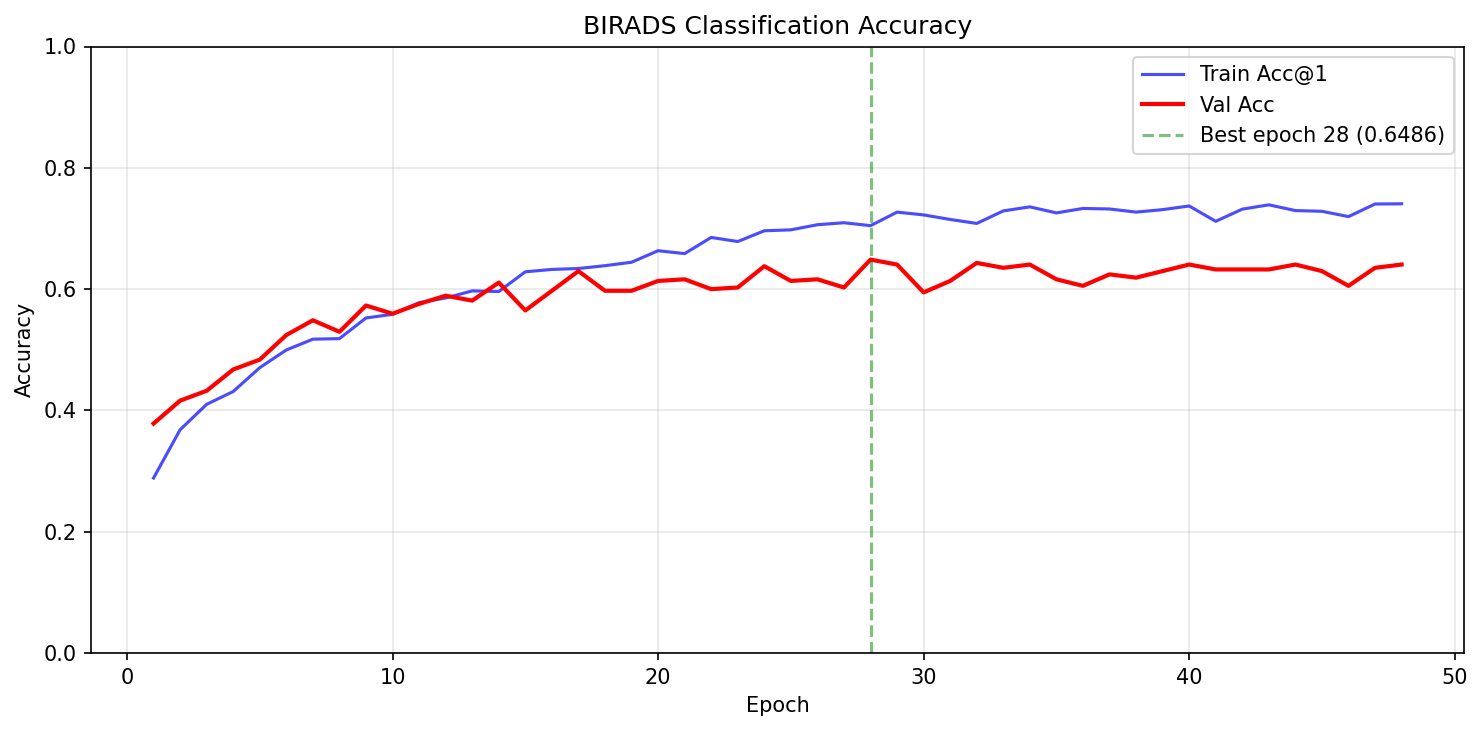
\includegraphics[width=0.85\textwidth]{images/accuracy.png}
\caption{BI-RADS 分类准确率曲线（绿色虚线标注最佳 epoch）}
\label{fig:accuracy}
\end{figure}

分析要点：
\begin{itemize}
    \item 训练集 Top-1 准确率稳步上升至约 74.1\%，表明模型在训练数据上学习充分。
    \item 验证集准确率最终达到 64.05\%，绿色虚线标注了最佳 epoch（第 29 轮）的峰值位置。
    \item 训练与验证准确率之间存在约 10 个百分点的差距，提示存在一定程度的过拟合。可通过增加 MixUp 概率、提高标签平滑系数或进一步降低模型容量来缩小这一差距。
\end{itemize}

\subsection{特征检测性能可视化}

\subsubsection{特征检测 IoU 曲线}

图 \ref{fig:iou} 展示了四项特征正样本（特征存在）边界框的交并比（IoU）随训练轮数的变化。

\begin{figure}[htbp]
\centering
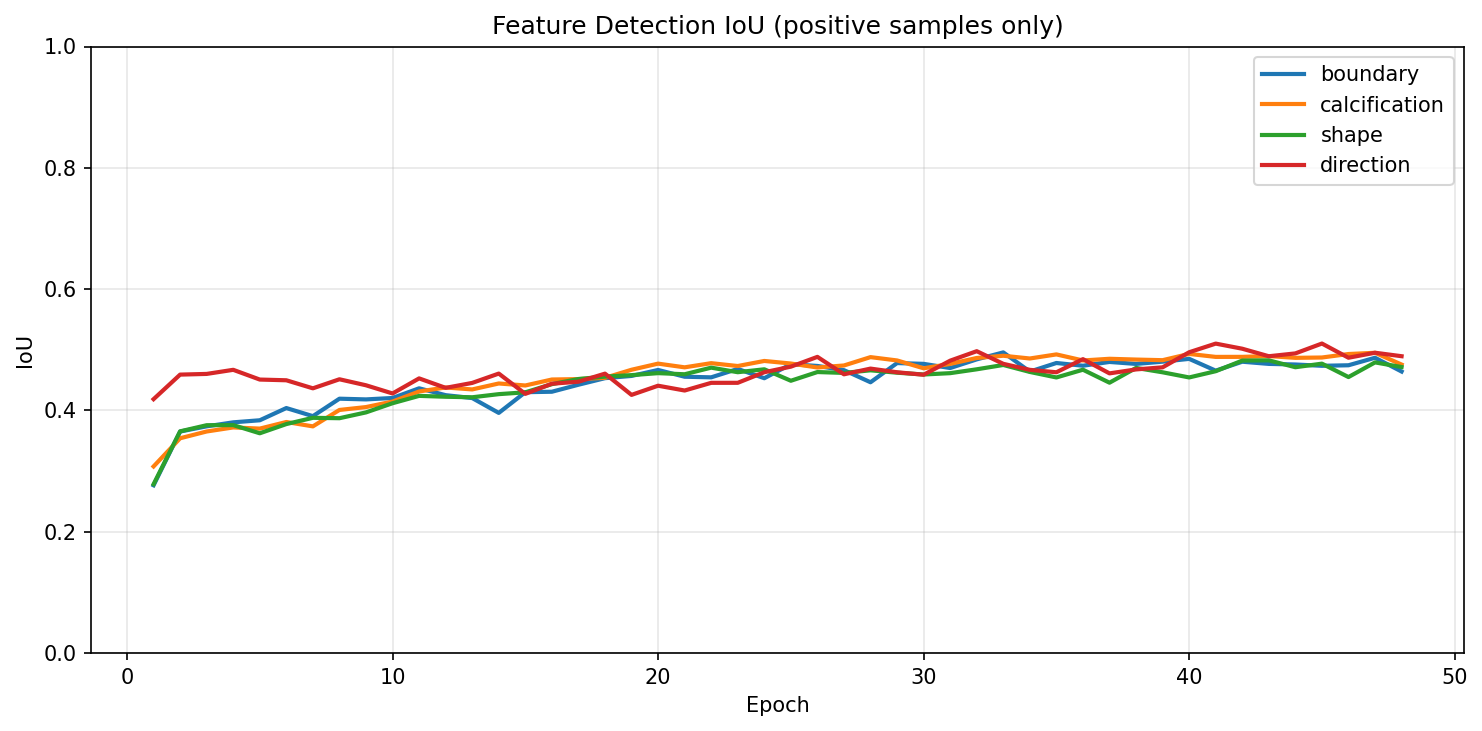
\includegraphics[width=0.85\textwidth]{images/iou_curves.png}
\caption{四项特征检测 IoU 曲线（仅统计正样本）}
\label{fig:iou}
\end{figure}

四项特征的 IoU 均收敛至 0.46--0.49 区间，定位精度整体一致。其中钙化（橙色）的 IoU 最高（约 0.48），方向（红色）的 IoU 略低（约 0.46）。训练初期（前 10 轮）IoU 快速提升，之后缓慢改善趋于平稳，表明检测头的定位能力已接近当前架构的上限。

\subsubsection{特征分类完整指标}

图 \ref{fig:feature_metrics} 以 2×2 子图的形式展示了四项特征分类的精确率、召回率、F1 分数和特异性指标。

\begin{figure}[htbp]
\centering
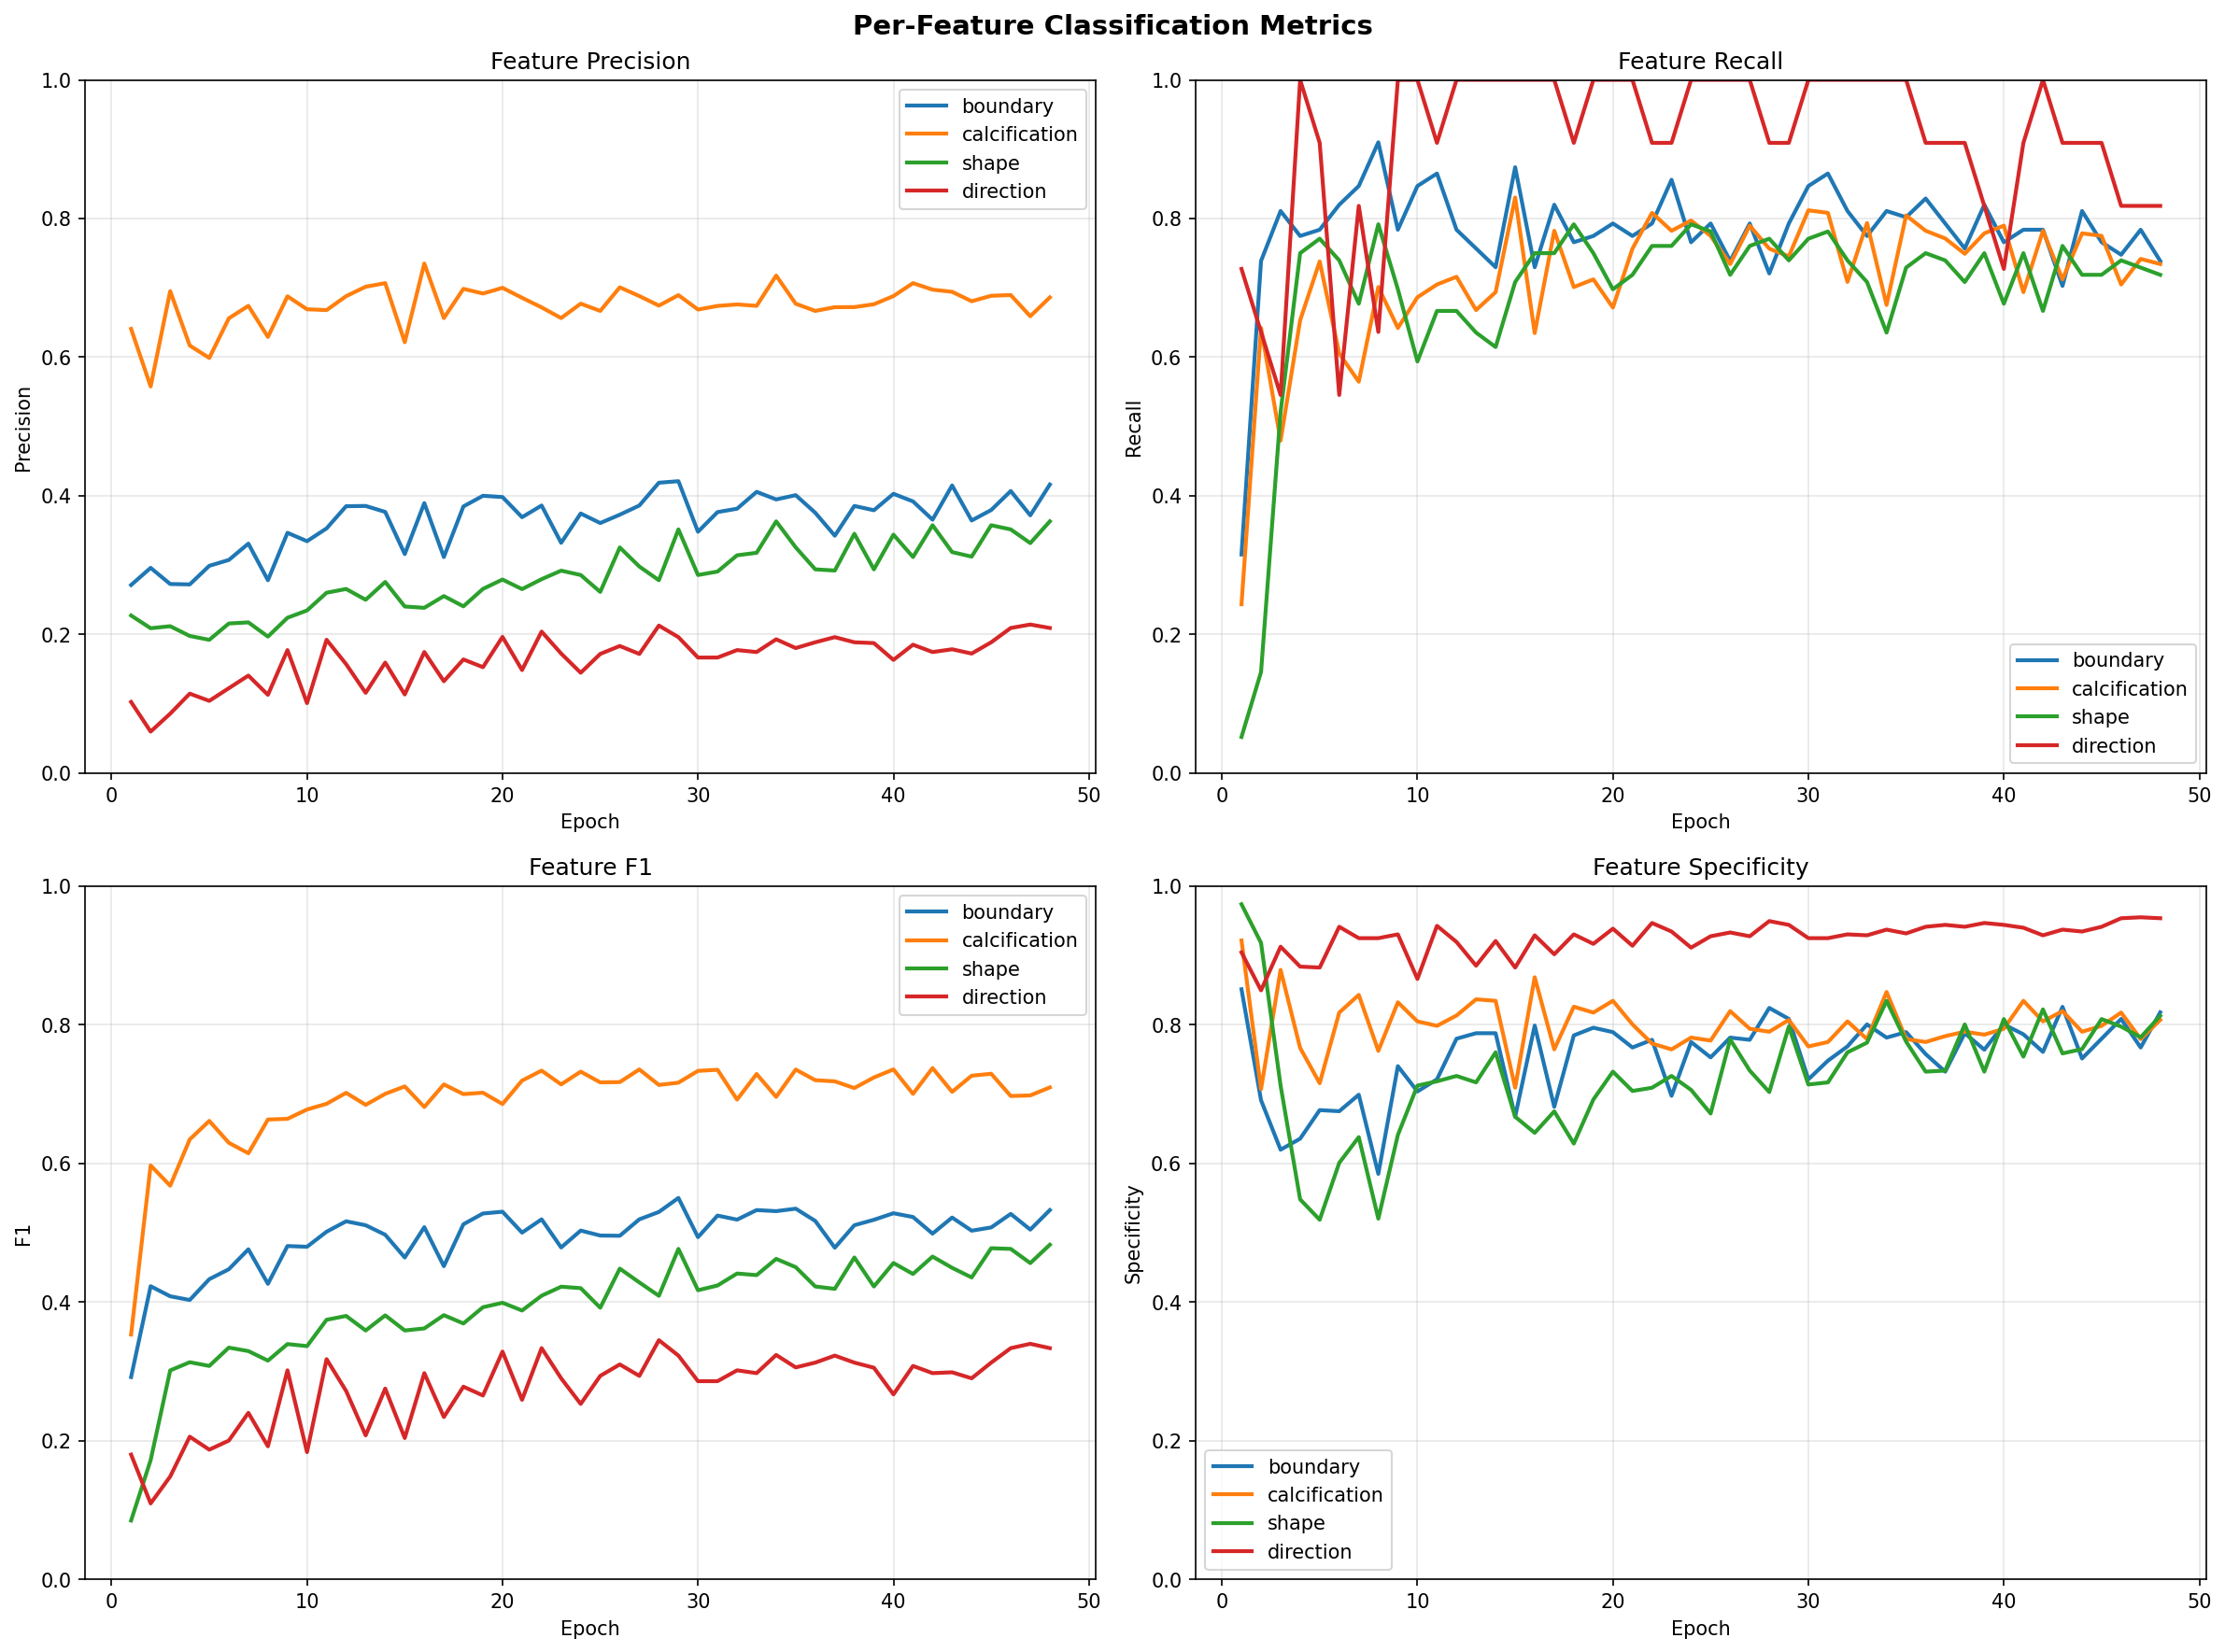
\includegraphics[width=0.95\textwidth]{images/feature_cls_metrics.png}
\caption{特征分类完整指标：Precision / Recall / F1 / Specificity}
\label{fig:feature_metrics}
\end{figure}

关键发现：
\begin{itemize}
    \item \textbf{精确率（Precision）}：钙化最高（约 0.69），方向最低（约 0.20），方向检测的假阳性问题最为突出。
    \item \textbf{召回率（Recall）}：方向最高（约 0.91），说明模型对方向正样本高度敏感，但精确率过低导致大量误报。
    \item \textbf{F1 分数}：钙化最优（约 0.72），方向最差（约 0.33）。方向的高召回被低精确率严重拖累。
    \item \textbf{特异性（Specificity）}：四项特征均在 0.79--0.94 之间，方向的特异性最高（0.94），与低精确率形成反差，进一步证实假阳性问题的严重性。
\end{itemize}

\subsubsection{特征检测 Loss 分解}

图 \ref{fig:det_breakdown} 展示了四项特征各自独立的分类损失（cls loss）与边界框损失（bbox loss）分解。

\begin{figure}[htbp]
\centering
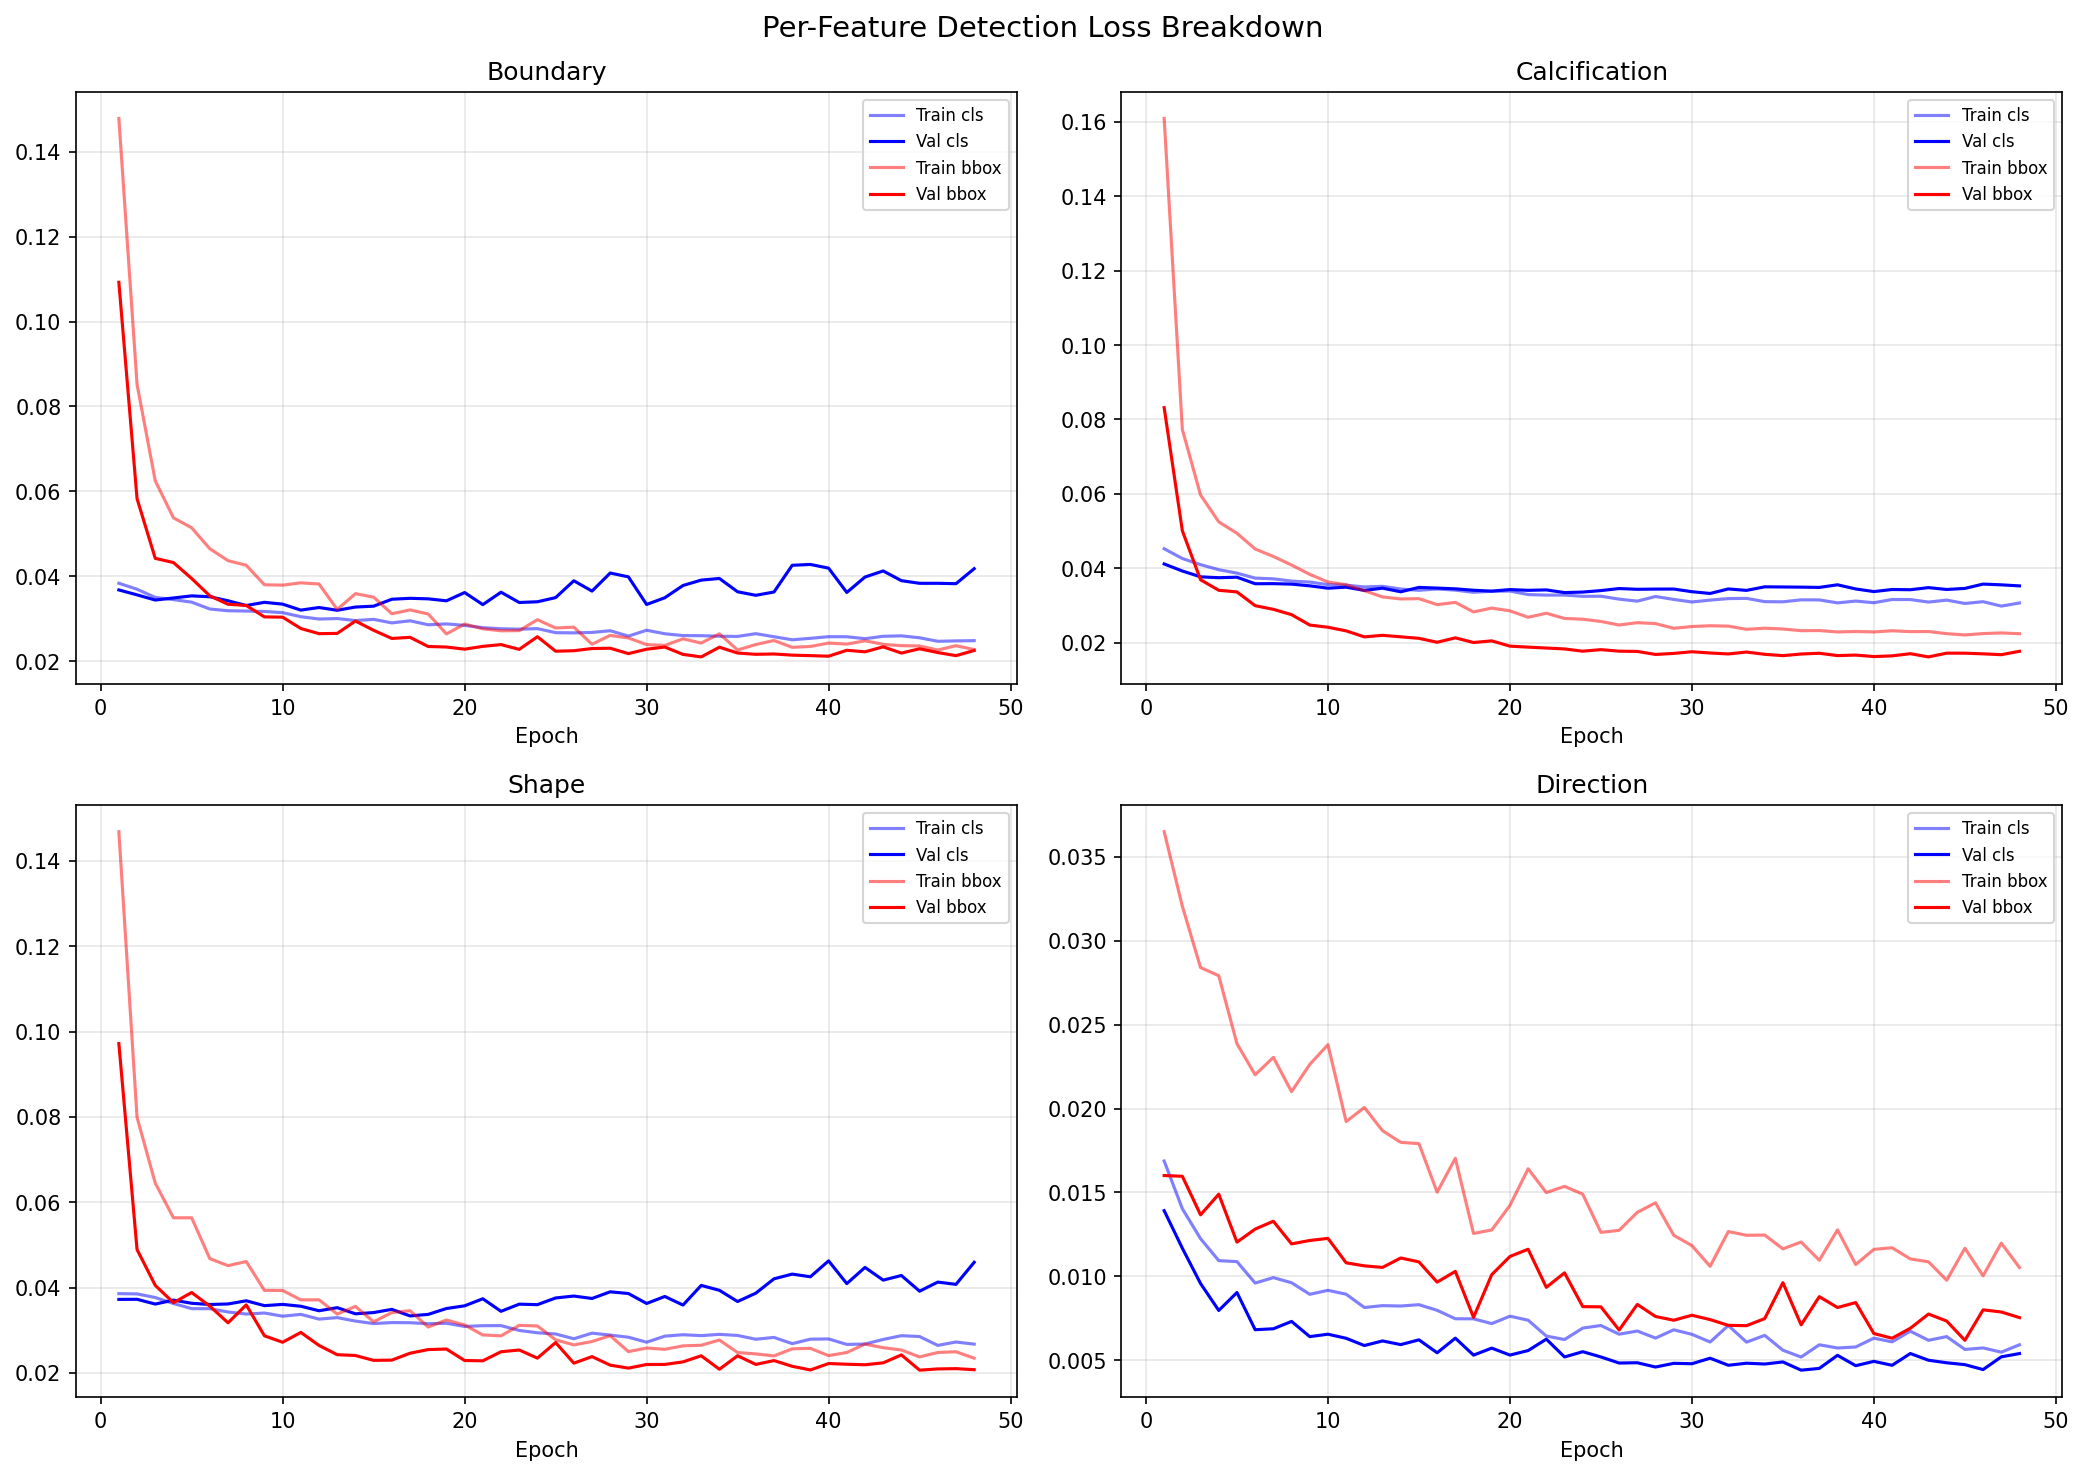
\includegraphics[width=0.95\textwidth]{images/det_breakdown.png}
\caption{特征检测 Loss 逐特征分解（蓝线：分类 Loss，红线：边界框 Loss）}
\label{fig:det_breakdown}
\end{figure}

从图中可以看出，边界（boundary）和形状（shape）的分类损失收敛值相对较高，反映了正负样本严重不平衡导致的分类困难。方向（direction）的分类损失最低（约 0.005），说明模型在此特征上分类过于偏向负样本，这也是假阳性问题的根源。而所有特征边界框损失均在稳步下降至 0.01--0.02 之间，定位能力持续改善。

\subsubsection{检测 AP@0.5 曲线}

图 \ref{fig:det_ap} 展示了检测 AP@0.5（类别正确且 IoU＞0.5 的检出率）随训练轮数的变化。

\begin{figure}[htbp]
\centering
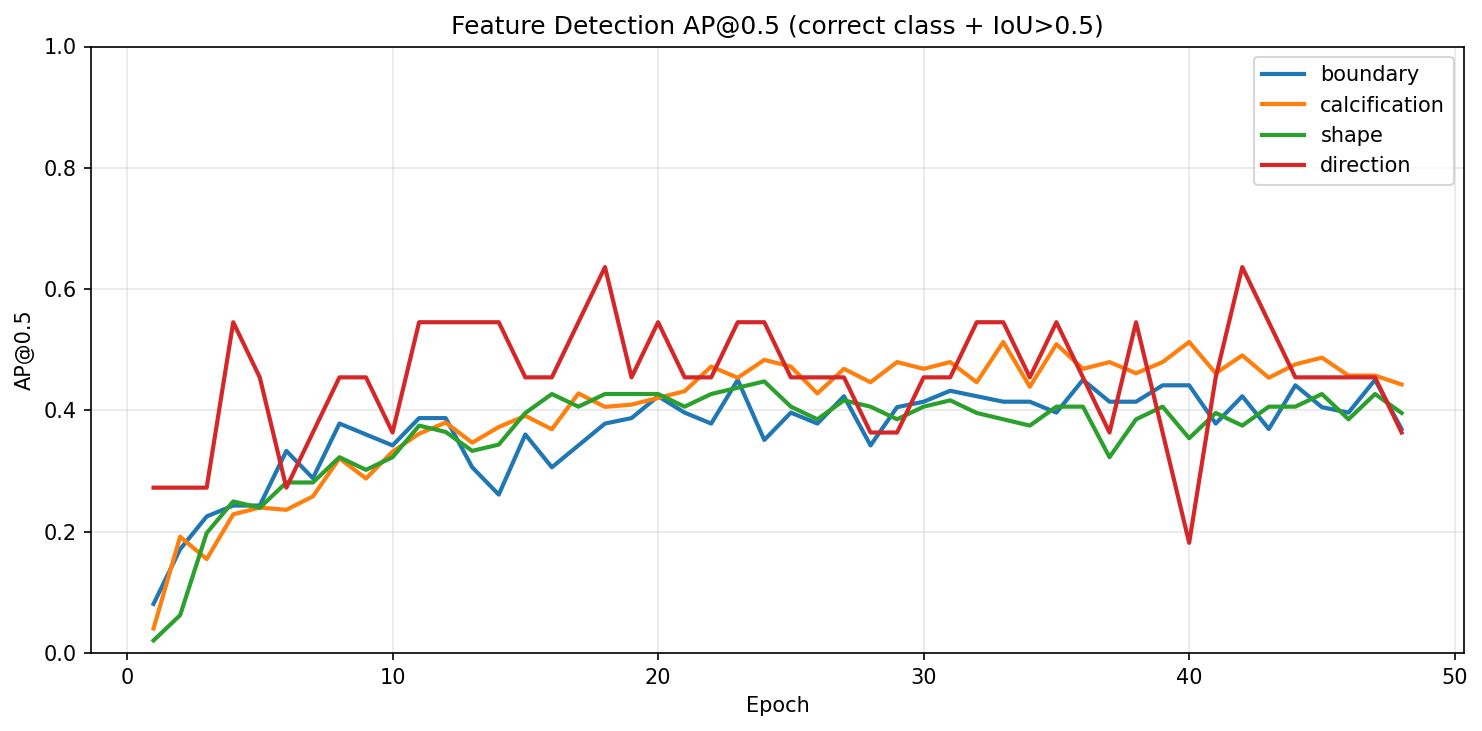
\includegraphics[width=0.85\textwidth]{images/detection_ap.png}
\caption{检测 AP@0.5 曲线（综合衡量分类精度与定位精度）}
\label{fig:det_ap}
\end{figure}

钙化（橙色）的 AP@0.5 最高（约 0.48），是综合分类与定位表现最优的特征。方向（红色）AP@0.5 仅约 0.36，边界（蓝色）约 0.41，形状（绿色）约 0.40。方向与形状的低 AP@0.5 主要由分类精确率过低导致，改进方向为提高 Focal Gamma 值、引入在线困难样本挖掘（OHEM）。

\subsection{学习率调度与训练效率}

图 \ref{fig:lr} 展示了 CosineAnnealing 配合 5 轮 Linear Warmup 的学习率调度曲线。

\begin{figure}[htbp]
\centering
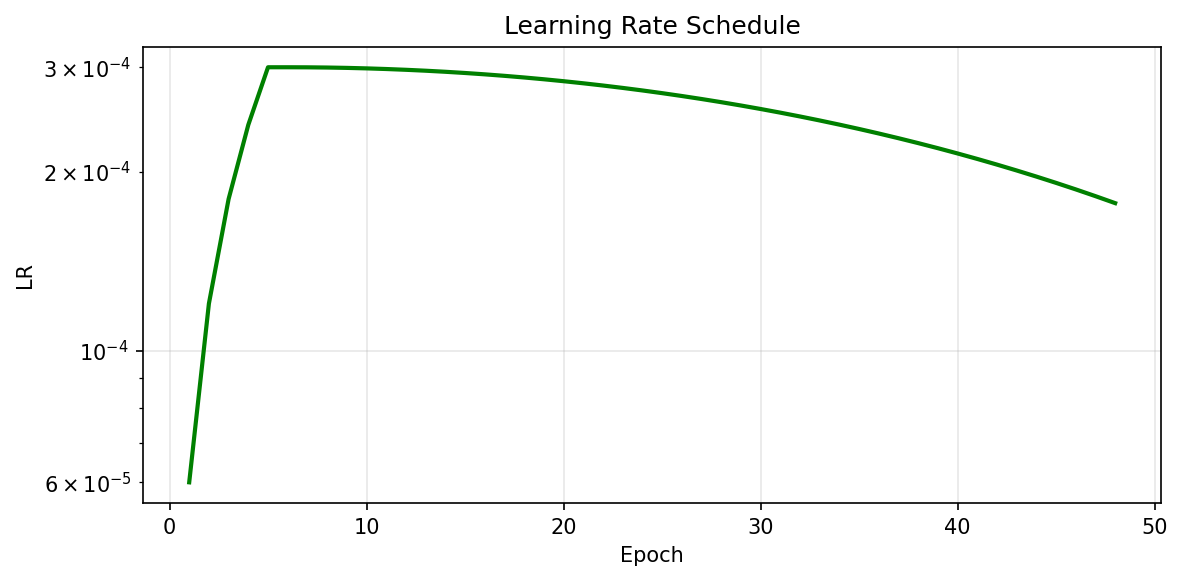
\includegraphics[width=0.8\textwidth]{images/lr_curve.png}
\caption{学习率调度曲线（Log 尺度 Y 轴）}
\label{fig:lr}
\end{figure}

训练采用了余弦退火（Cosine Annealing）学习率调度策略，配合 5 个 epoch 的线性预热（Linear Warmup）。预热阶段学习率从 0 线性增长至基础学习率 \(3 \times 10^{-4}\)，之后沿余弦曲线平滑衰减。实际训练在第 48 轮因早停触发而终止，此时学习率约为 \(1.77 \times 10^{-4}\)，模型已收敛至最优解附近。

\subsection{混淆矩阵}

图 \ref{fig:confusion} 展示了四项超声特征分类的混淆矩阵，直观呈现了各特征真阳性、真阴性、假阳性、假阴性的样本分布。

\begin{figure}[htbp]
\centering
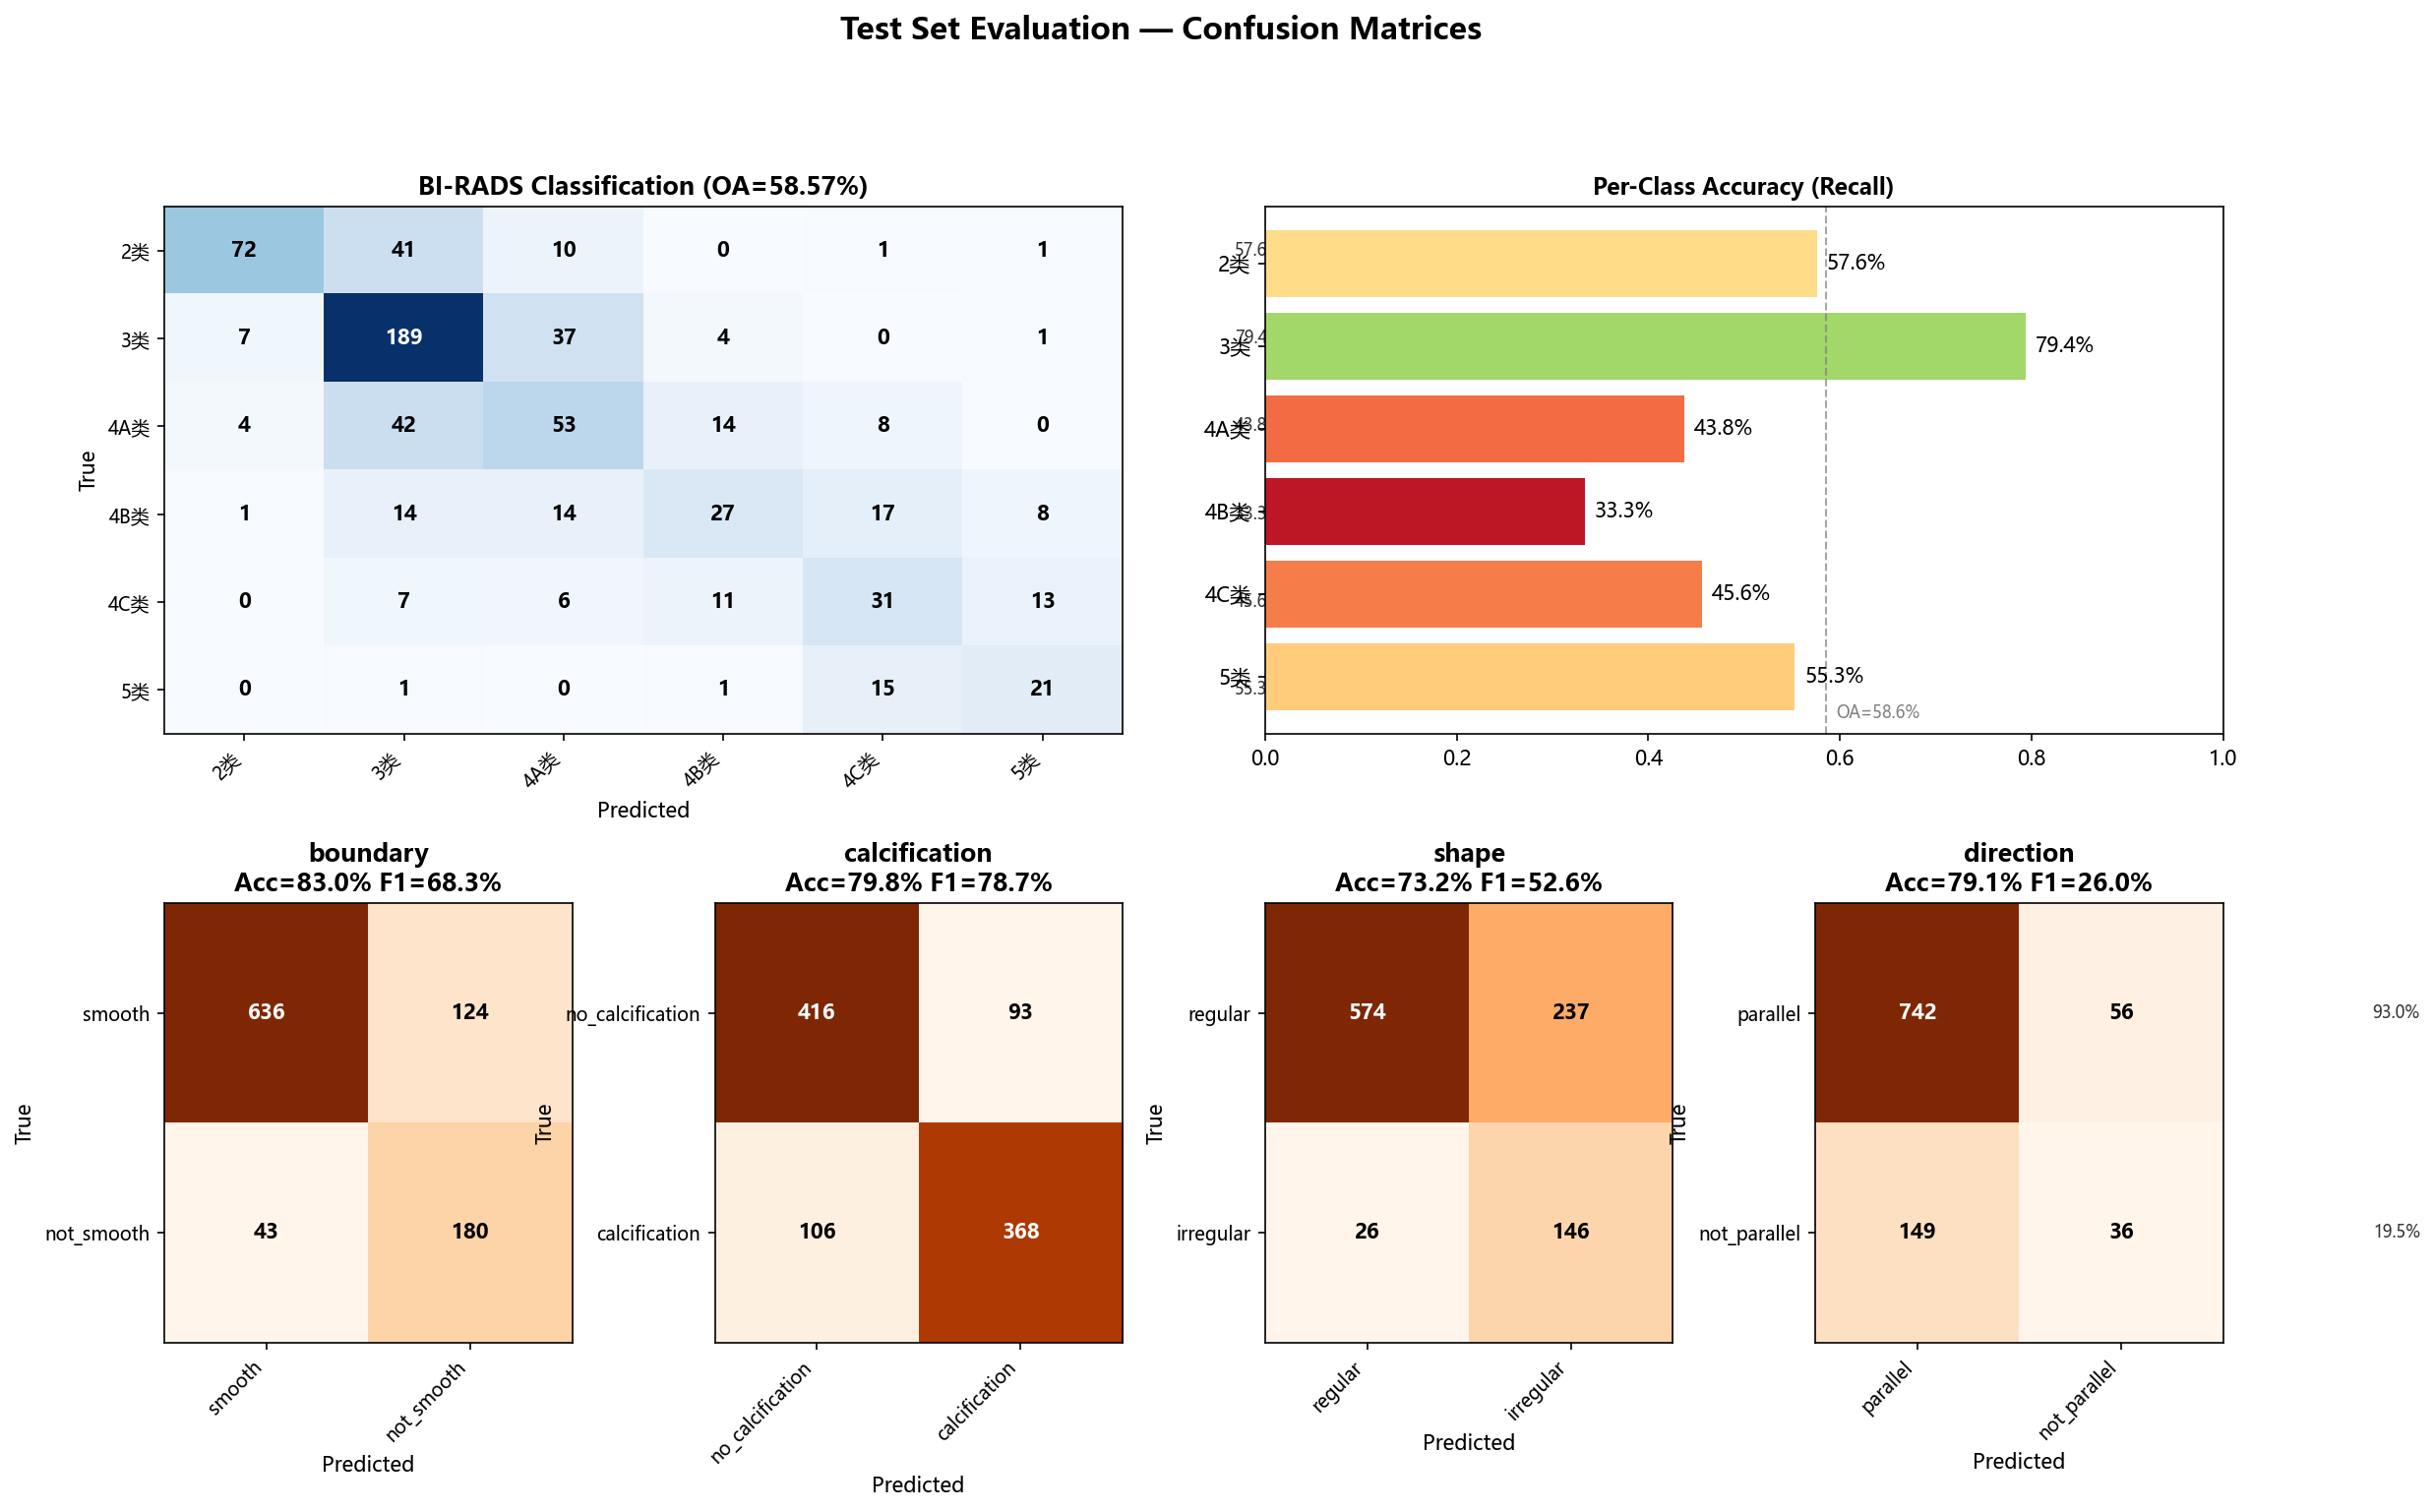
\includegraphics[width=1\textwidth]{images/confusion_matrices.png}
\caption{四项超声特征分类混淆矩阵}
\label{fig:confusion}
\end{figure}

由混淆矩阵可以直观验证：
\begin{itemize}
    \item \textbf{钙化}：混淆矩阵分布最为均衡，假阳性和假阴性数量均较低，与 F1 分数最高（71.63\%）的结论一致。
    \item \textbf{方向}：假阳性（将阴性误判为阳性）数量显著偏高，假阴性（将阳性漏判为阴性）数量很低，与精确率 19.61\%、召回率 90.91\% 的数据特征完全吻合。
    \item \textbf{形状}：假阳性问题同样突出，但程度较方向略轻。
    \item \textbf{边界}：各项指标处于四者中间水平，性能相对均衡。
\end{itemize}

\subsection{模型性能总结}

综合以上分析，本模型在乳腺超声 BI-RADS 分类与特征检测任务上取得了初步成果，算法性能得分 \(A = 72.20\%\)。主要性能瓶颈集中在方向（direction）和形状（shape）特征的检测精确率过低（分别为 19.61\% 和 35.15\%），导致假阳性率偏高。

\end{document}
